\section{Provenance}
In the Oxford dictionary, \emph{provenance} is defined as ``the place of origin or earliest known history of something''. Provenance plays an important role in many aspects of our daily lives. For example, in \emph{food} industry, before purchasing a bottle of fruit juice, a customer would like to know about its origin, ingredients, methods of collecting, storing and processing fruits, etc. In \emph{art}, the provenance information of a painting such as authorship, material, painting time and the story behind the painting greatly decides its value. In computer systems, the provenance of a piece of data is defined as ``the process that led to that piece of data''~\cite{Moreau2011}. \add{It contains information about the input data, the output data, and the configuration of the executing program used to process the data.}

We broadly categorize provenance into two groups. \add{The first group, \emph{data provenance}, relies on the previous definition of provenance, focusing on the derivation history of derived data including the source information of data and the process that produced it. This type of provenance is often emphasized in data-intensive fields such as scientific workflows and databases. The second group, \emph{analytic provenance}, usually happens in the context of visualization and sensemaking. It focuses on the interactive data exploration and reasoning processes driven by sensemaking including the provenance of visualizations used, interactions performed, analytical insights found and the conclusion and rationale behind them.} Next, we discuss data provenance in different fields, notably scientific workflows, databases and semantic webs. Analytic provenance will be discussed in \autoref{sec:lr-analytic-provenance}.

%\subsection{Data Provenance}
%\label{sub:lr-data-provenane}
Scientific experiments may consist of thousands of steps, with each step involving distributed data sources and computational data models~\cite{Gil2007}. Workflows have been used to facilitate the assembly, automation and management of such experiments. Notable scientific workflow systems with provenance enabled include Tarvena~\cite{Zhao2008}, Kepler~\cite{Bowers2006} and VisTrails~\cite{Bavoil2005}. Provenance plays an important role in scientific workflows, aiming to support data interpretation, reproduction of experiment results, troubleshooting and optimization~\cite{Miles2007}. \add{Zhao, Wilde and Foster~\cite{Zhao2006} discuss two types of provenance in workflows: \emph{prospective provenance} -- focusing on the workflow design, and \emph{retrospective provenance} -- focusing on the workflow execution.} The provenance of long and complex workflows is huge, thus pose challenges in storing, querying, and making sense of such data~\cite{Davidson2007}.

Curated databases are populated and updated with a great deal of human effort, typically published on the web~\cite{Buneman2008}. A well-known example is Wikipedia -- a free Internet encyclopedia that allows its users to edit almost any article accessible. Each record in these databases, such as a Wikipedia article, may be edited by many users and referred to other internal and external sources. This produces problems in attribution and provenance: who edited what at when. Research in database provenance can be characterized into a why-where-how framework~\cite{Cheney2007}. \emph{Why}-provenance focuses on the lineage of the output: for each tuple $t$ in the output, the lineage of $t$ is a set of tuples in the input data that helps produce $t$~\cite{Cui2000}. \emph{How}-provenance concerns how the output tuple $t$ is derived from the query~\cite{Green2007}. Finally, \emph{where}-provenance describes specific locations, or cells in relational databases, of the input data that contribute to the query output~\cite{Buneman2001}. To compute these types of provenance, two general approaches have been introduced~\cite{Buneman2008}. An \emph{eager} approach adjusts the query to pass the extra provenance information to the output. Whereas, a \emph{lazy} approach computes provenance on demand.

Data provenance research in scientific workflows and databases has mainly focused on closed systems, which have full access to the data and its provenance. Modern applications with service-oriented~\cite{Papazoglou2007} and cloud-computing~\cite{Buyya2009} architectures bring challenges in tracking and exchanging provenance information across systems. The \emph{Open Provenance Model} is designed to address these challenges~\cite{Moreau2011}. It also supports a digital representation of provenance for any objects, whether produced by computer systems or not. Three types of objects are defined in the model for building this representation. An \emph{artifact} is a state that can be a digital or physical object. A \emph{process} is a series of actions performed on or caused by artifacts, and resulting in new artifacts. An \emph{agent} acts as a catalyst of a process, managing its execution. Different types of causal relationships can be added between these nodes, forming a \emph{provenance graph} as shown in \autoref{fig:lr-provenance-graph}.

\begin{figure}[!htb]
	\centering
	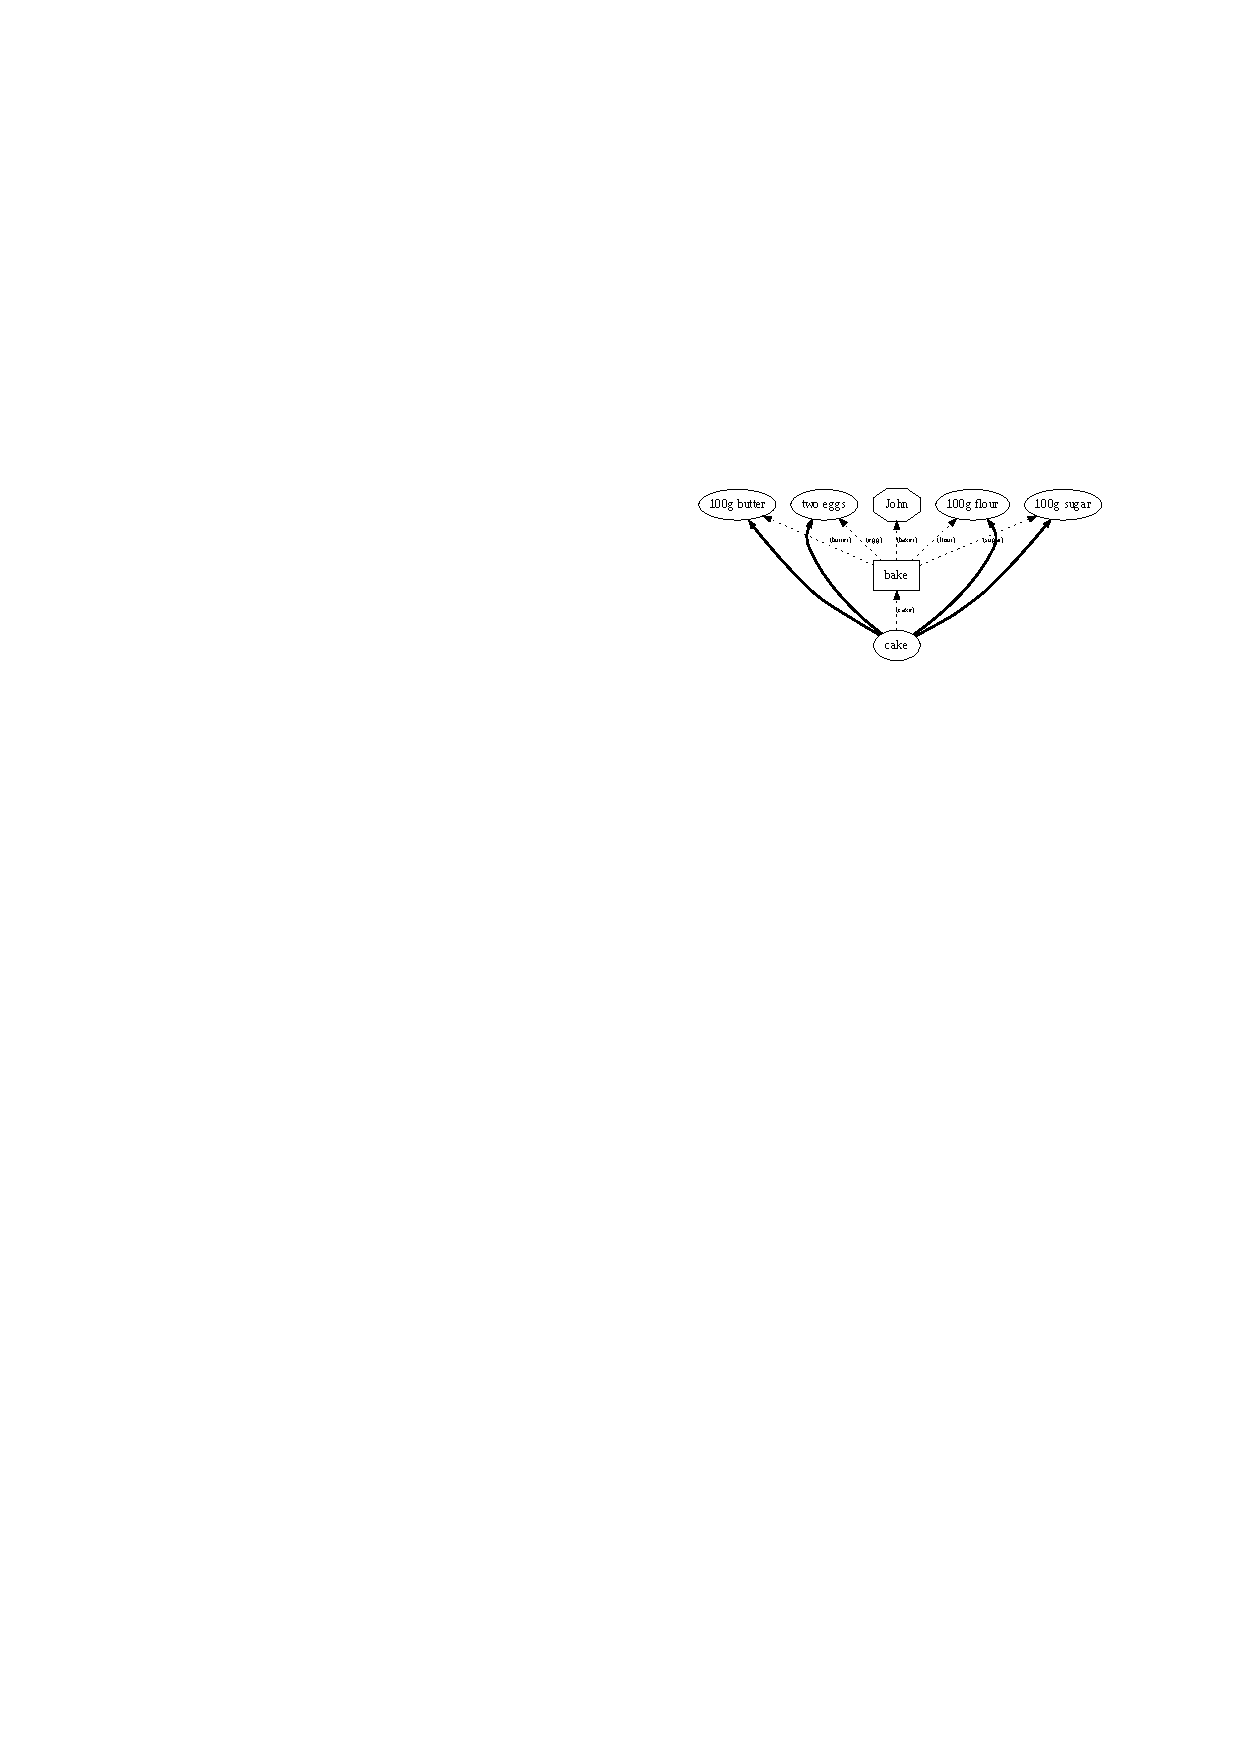
\includegraphics[width=\linewidth]{provenance-graph}
	\caption{A provenance graph for ``cake baking'' using the Open Provenance Model. The cake (artifact) was baked (the process) by John (the agent) using ingredients including butter, eggs, flour and sugar (artifacts). \is{Moreau2011}}
	\label{fig:lr-provenance-graph}
\end{figure}

The Open Provenance Model has been implemented in many systems, including notable scientific workflows such as Tarvena~\cite{Zhao2008}, Kepler~\cite{Bowers2006} and VisTrails~\cite{Bavoil2005}. The model is general and can be extended in both the structure and vocabulary to represent domain-specific problems. \emph{D-profile}~\cite{Groth2011} describes an extension of the model for representing provenance in distributed systems. ProveML~\cite{Walker2013} is another extension for recording the provenance of data, analytical process and interpretations in human terrain visual analytics.

\add{The \emph{PROV} set of specifications, produced by the World Wide Web Consortium, is designed to promote the publication of provenance information on the Web and support the interchange of provenance across diverse provenance management systems~\cite{Missier2013}. The PROV-DM is the conceptual data model that forms a basis of PROV and is based on the aforementioned open provenance model. PROV also includes other parts such as PROV-CONSTRAINTS, a set of constraints applying to the data model to impose rules for consistency and validity of provenance.}